% ~ 6 pages
\chapter{Theoretical Background}
\label{sec:theory}

In this chapter the theoretical background for the studies in this thesis is
provided. First the Standard Model of particle physics is introduced and its
problems discussed. Then physics of tau leptons is discussed with a focus on
hadronic decays of the tau lepton.

\section{The Standard Model of Particle Physics}

The Standard Model of particle physics describes the current understanding of
elementary particles and interactions between them. The Standard Model has been
extensively probed since its origin and shows excellent agreement with
experimental results. However, it does not offer a full description of particle
physics as it does not explain interactions of massive particles via gravity.

In Figure~\ref{fig:sm_particles} the elementary particles of the SM are shown.
They can be divided into the fermions consisting of particles with spin-half and
gauge with spin-1. In 2012 the ATLAS and CMS experiment at the Large Hadron
Collider discovered a new scalar boson with a mass
of~$m_\text{H} \approx \SI{125}{\GeV}$~\cite{higgs_atlas, higgs_cms}, which is
called the Higgs boson (SM like).

\begin{figure}[htb]
  \centering
  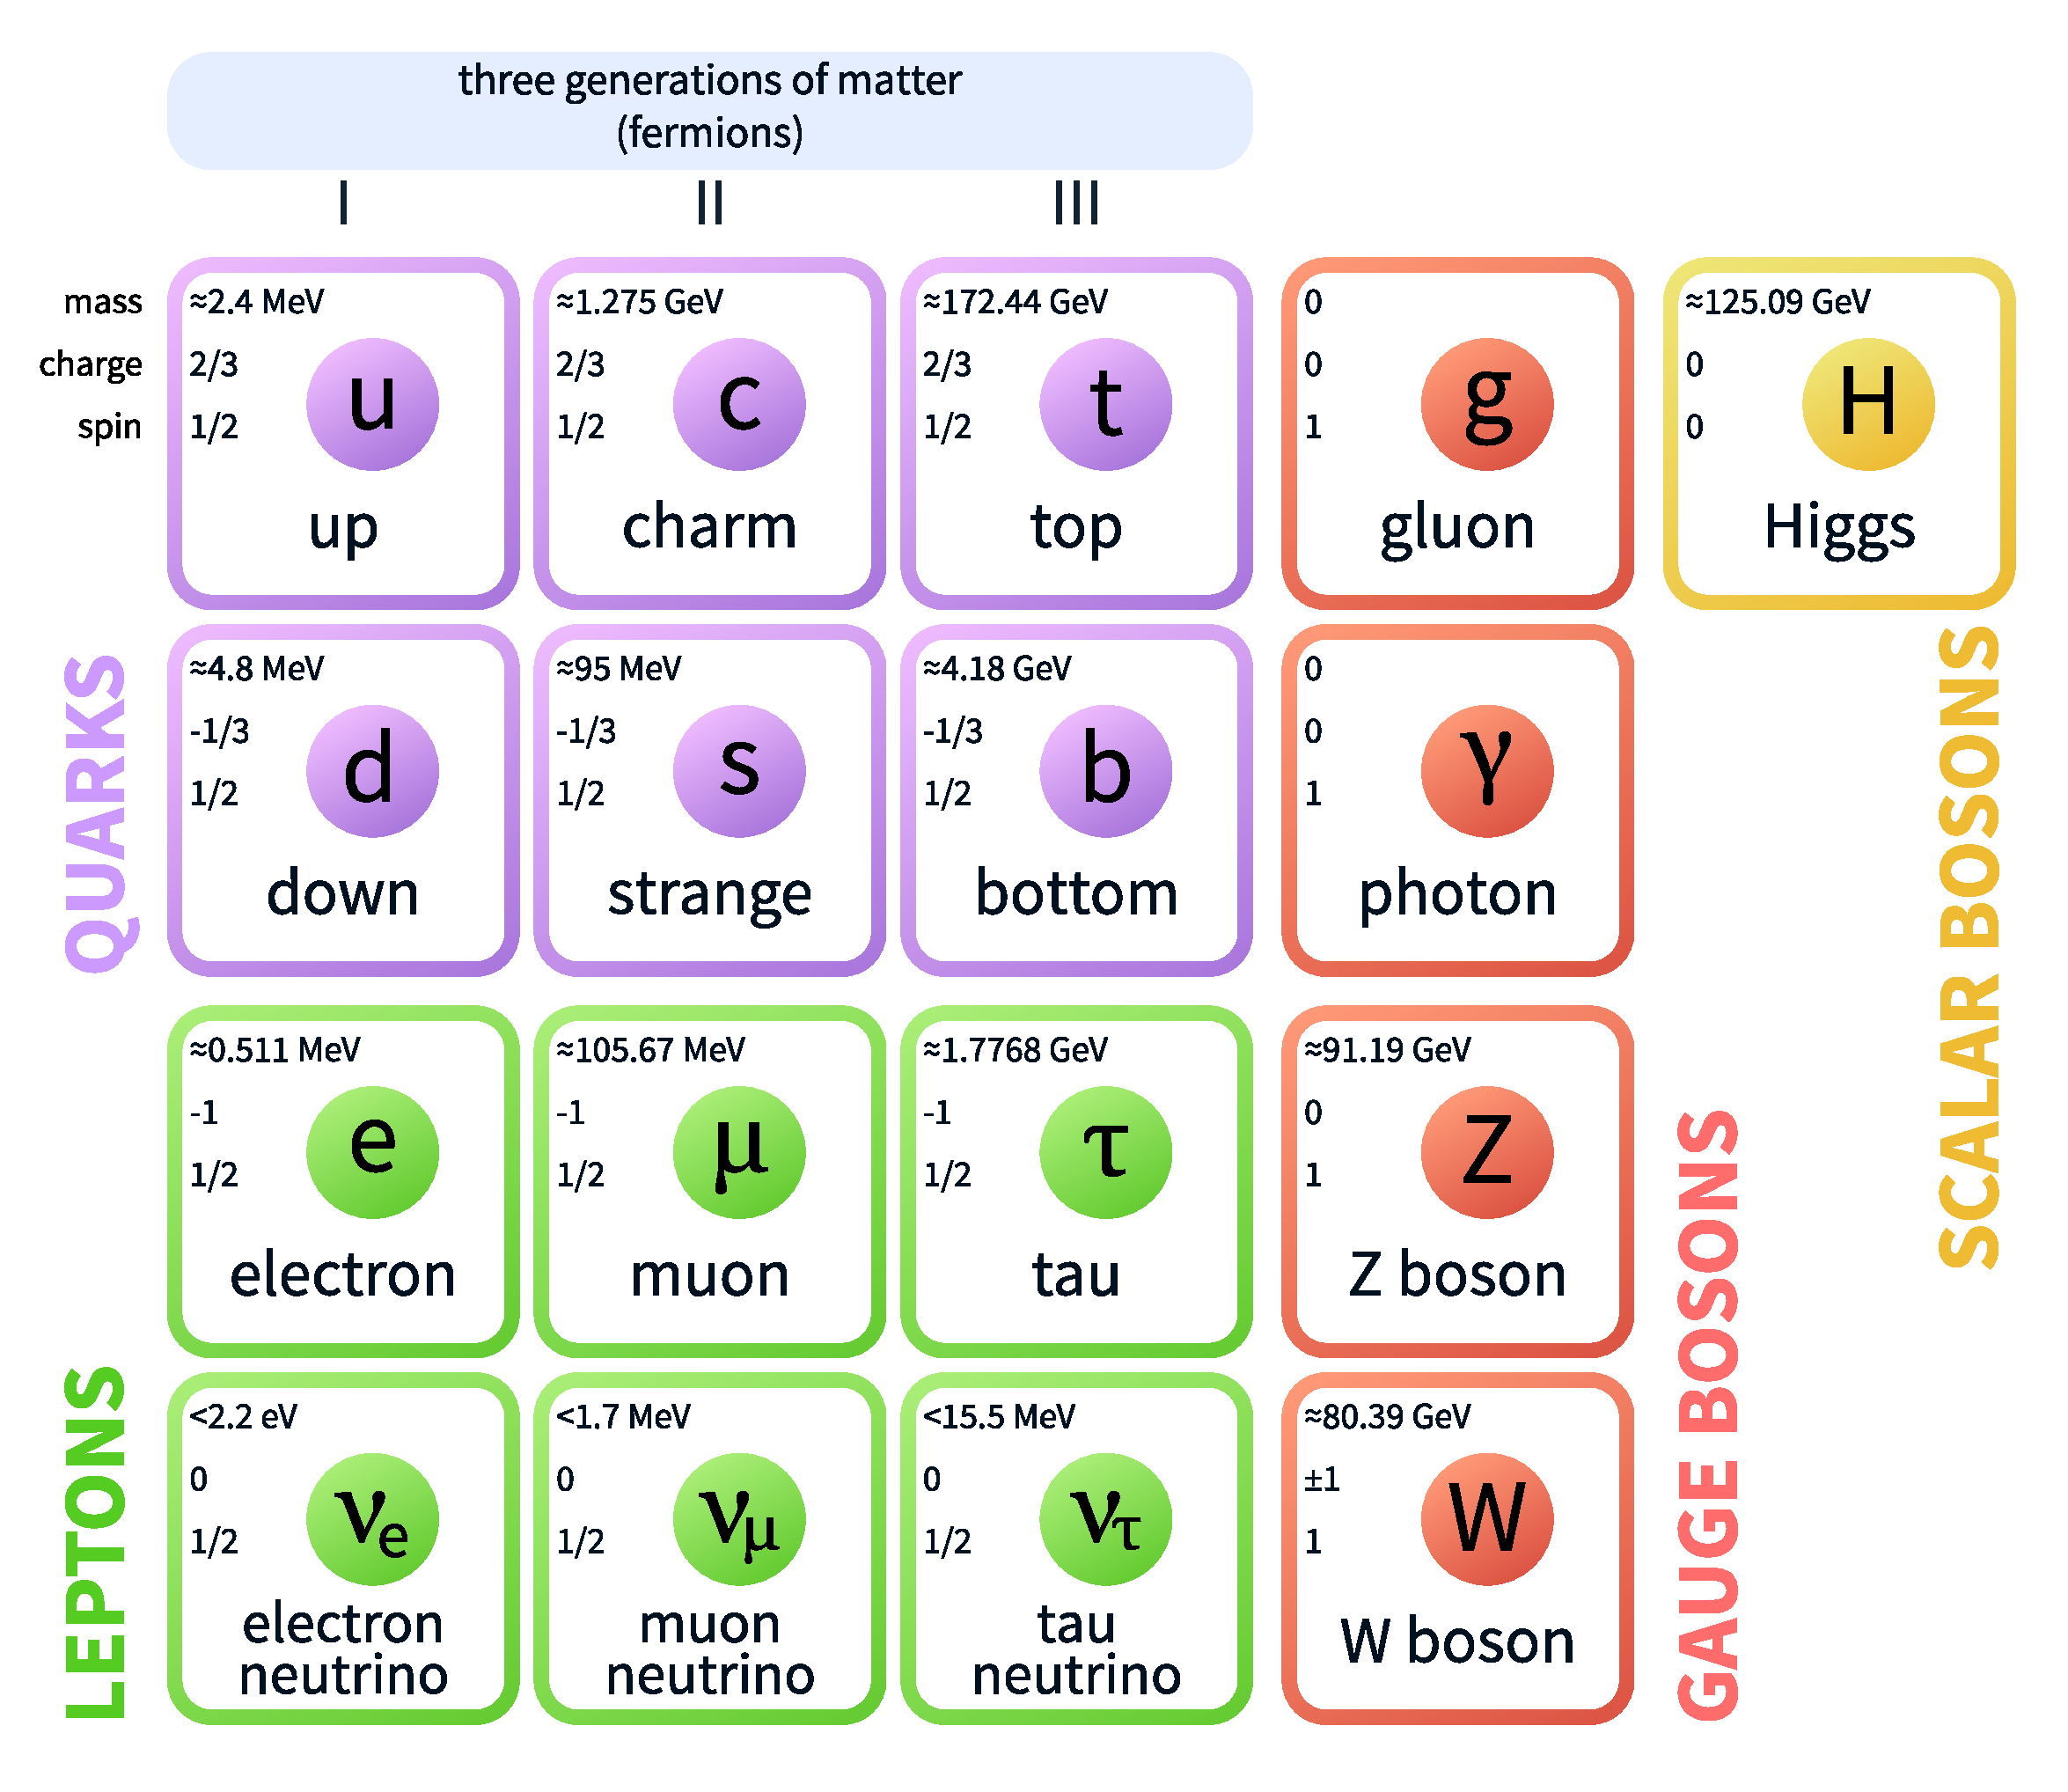
\includegraphics[width=0.7\textwidth]{./figures/theory/sm_particles.pdf}
  \caption{Particles of the Standard Model. Image modified from
    Ref.~\cite{sm_wiki}.}
  \label{fig:sm_particles}
\end{figure}

In the following the elementary particles and their interactions are described.
The fermions of the Standard Model form the observable matter. The dynamics of
fermions are described by the Dirac equation, while interactions between them
are mediated by the gauge bosons. The nature of these interactions is described
by quantum field theories and the local gauge principle. The fermions are
divided into up- and down-type quarks with a charge of~$\frac{2}{3}$
and~$-\frac{1}{3}$, respectively and leptons consisting of the charged leptons
and the neutrinos. The fermions are divided into three generations with
identical properties with the exception of their mass. The first generation
consisting of the electron, electron neutrino, up- and down-quark makes up most
of the matter in the low-energy universe. The quarks of the second and third
generation are produced in high-energy particle collisions. Each fermion has a
corresponding antiparticle with the same mass but with inverted additive quantum
numbers including the electric charge.

The strong interaction between quarks is described by quantum chromodynamics.
The exchange particle of the strong force is the massless gluon, which couples
to the so called color charge. The quarks as well as the gluons carry color
charge allowing $qqg$-vertices as well as gluon self-coupling in triple and
quartic gluon vertices. Experimentally, free quarks are not observed but only
color-neutral bound states called hadrons. This is known as colour confinement
and leads to the formation of collimated jets of hadrons in processes creating
high-energy quarks or gluons.

The electromagnetic interaction between particles carrying electric charge is
described by quantum electrodynamics. The mediating gauge boson is the massless
photon, which couples to charged particles including quarks, charged leptons and
the $W^\pm$~boson.

The weak interaction is mediated by the massive $Z^0$ and $W^\pm$~bosons, which
couple to the weak charges carried by all fermions. Additionally, couplings
between the weak bosons itself are allowed. The weak interaction violates
$\mathcal{P}$ and $\mathcal{CP}$ symmetry. The weak charged-current interaction
is mediated by the $W^\pm$~boson and couples to chiral left-handed particles and
chiral right-handed antiparticles. The weak charged-current allows flavour
changes in the quark sector. In contrast to this, the weak neutral-current
interaction mediated by the $Z^0$~boson does not allow flavour changes. The
$Z^0$ couples to both left- and right-handed particles although with different
strength.

The electromagnetic and weak interactions are unified in the electroweak theory
developed by Glashow, Salam and Weinberg~\cite{glashow, salam, weinberg}. The
local gauge symmetry~$\mathrm{SU}(2)_\text{L}$ generating the weak
charged-current interaction and the $W^+$, $W^-$ boson fields as well as a
neutral field $W^{(3)}$ coupling to chiral left-handed particles. The
electroweak unification introduces a $\mathrm{U}(1)_Y$, where~$Y = 2 (Q - T_3)$
is the weak hypercharge depending on the electric charge~$Q$ and the third
component of the weak isospin~$T_3$. The~$\mathrm{U}(1)_Y$ symmetry generates a
neutral field~$B$ that mixes with~$W^{(3)}$ giving rise to the photon and $Z^0$
boson fields, thus combining the weak and the electromagnetic interaction.

The non-vanishing masses of the $W^\pm$ and $Z^0$ bosons break the local gauge
invariance of the electroweak theory when introducing a mass term into the
Lagrangian. To maintain the gauge principle a different approach called the
Higgs mechanism~\cite{englert_brout, higgs} is introduced so that the weak
bosons can acquire their mass in a process called \emph{spontaneous symmetry
  breaking}. For this a doublet of complex scalar fields with non-vanishing
vacuum expectation value is introduced. This breaks the symmetry of the
Lagrangian and introduces four degrees of freedom. Three are absorbed into the
$W^+$, $W^-$ and $Z^0$ bosons giving them mass. The remaining neutral and scalar
component becomes the physical Higgs boson. The Higgs mechanism is also used to
generate masses of the fermions, however neutrinos are assumed to be massless in
the Standard Model.

\subsection{Problems of the Standard Model}

The Standard Model predicts and has been extensively tested. However, some
phenomena remain unexplained in the Standard Model:
\begin{description}
\item[Gravity] Currently, no complete and consistent quantum field theory of
  gravity exists. Therefore, the Standard Model cannot describe the
  gravitational interaction between massive particles.

\item[Dark matter] The Standard Model does not provide a weakly interacting
  massive particle that explains both the observed gravitational interaction of
  dark matter as well as the large-scale structure of the observable Universe.

\item[Origin of neutrino masses] The discovery of neutrino
  oscillations~\cite{superk_neutrino, sno_neutrino_1, sno_neutrino_2} show that
  neutrinos have mass. The origin of this mass is not determined in the Standard
  Model. It can be generated using the Higgs mechanism making neutrinos Dirac
  particles. Another possibility is neutrinos being Majorana particles, in which
  case the seesaw mechanism could explain the experimentally observed mass scale
  of neutrinos.

\item[Matter--antimatter asymmetry] The baryon number and $\mathcal{CP}$
  violation required by the Sakharov conditions~\cite{sakharov} to explain the
  observed matter--antimatter asymmetry, cannot be provided in the Standard
  Model.

\item[Hierarchy problem] The Higgs boson mass is modified by radiative
  corrections due to fermionic and bosonic loops in the Higgs
  propagator~\cite{bettini}. At high energy scales the Higgs mass would be
  large, requiring fine-tuning of the contributions to the Higgs mass to keep it
  at the electroweak scale~\cite{thomson}. Supersymmetry offers a solution to
  this problem, cancelling the corrections.

\item[Unification of the forces] The couplings of the three interactions
  described in the Standard Model are of the same order of magnitude at the
  electoweak energy scale. They might converge at even higher energies,
  suggesting that the Standard Model is only a low-energy manifestation of a
  unified theory~\cite{thomson}.

\item[Number of parameters] A total of 26 free parameters consisting of 12
  fermion masses, 3 coupling constants, the vacuum expectation value of the
  Higgs field and mass of the Higgs boson, 6 mixing angles and 2 phases in the
  PMNS and CKM matrix and potentially a $\mathcal{CP}$~violating phase of the
  strong interaction, are needed to describe the Standard Model~\cite{thomson}.
  The large number of parameters is sometimes viewed as inelegant for describing
  a fundamental theory.
\end{description}
Explanation for these issues need to extend the Standard Model or introduce new
theories beyond the Standard Model, e.g.\ Supersymmetry or Grand Unified
Theories.

\section{Tau Leptons}


\todo[inline]{Define 1-prong, 3-prong and multi-prong.}

The tau lepton is the heaviest lepton in the Standard Model and an important
probe of physics at high energy scales, such as Higgs physics and physics beyond
the Standard Model. Hadronic decays make up approximately two-thirds of the
total branching ratio of tau decays and play an important part in the physics
programme of the ATLAS experiment.

\begin{figure}[ht]
  \begin{subfigure}[b]{0.47\textwidth}
    \centering
    \begin{overpic}{./figures/theory/tau_branching_pie_chart.pdf}
      \put (34, 83) {$\pi^- \nu_\tau$}
      \put (-1, 45) {$\pi^- \pi^0 \nu_\tau$}
      \put (19, 8) {$\pi^- 2 \pi^0 \nu_\tau$}
      \put (44.5, 2) {$2 \pi^- \pi^+ \nu_\tau$}
      \put (69, 6) {$2 \pi^- \pi^+ \pi^0 \nu_\tau$}
      \put (80, 15) {other}
    \end{overpic}
    \caption{Tau branching ratios \cite{pdg}. Adapted from
      Ref.~\cite{ikai_trigger}.}
    \todo[inline]{Fix wonky percentages for hadronic modes}
    \label{fig:tau_branching_ratios}
  \end{subfigure}\hfill
  \begin{subfigure}[b]{0.47\textwidth}
    \centering
    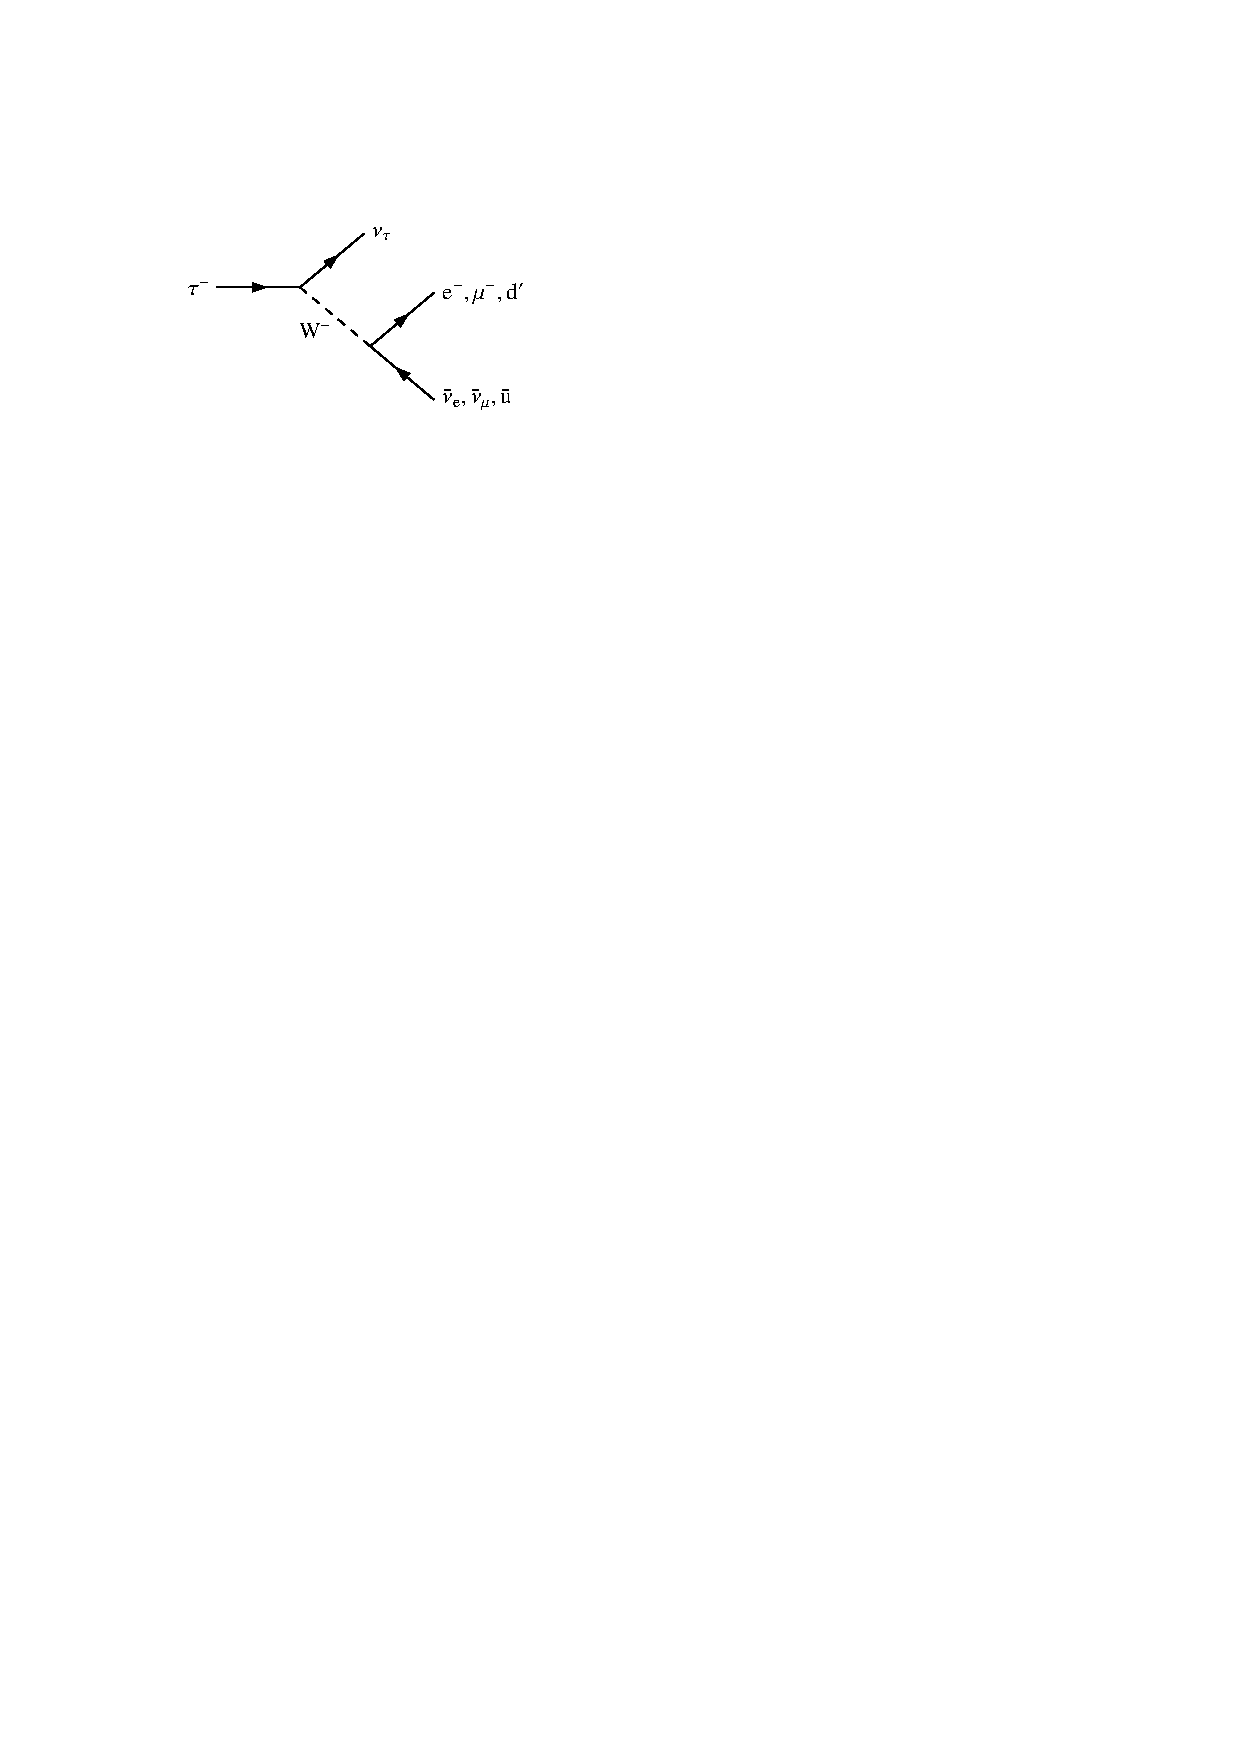
\includegraphics{./figures/theory/tau_decay_feynman.pdf}
    \caption{Feynman Diagram. Strangeness production is Cabibbo suppressed by a
      factor of $\sin^2\theta_\mathrm{c} / \cos^2\theta_\mathrm{c} \approx
      \frac{1}{20}$. Ignoring phase space considerations the tau decays to
      $\frac{1}{5}$ into electron or muon and corresponding antineutrino or into
      a down anti-up quark pair (3 colours).}
  \end{subfigure}
  \caption{Weak decay of the tau-lepton}
\end{figure}

\begin{itemize}
\item Discovery at SPEAR in 1975 [Check Citation]\cite{perl}
\item $m_\tau = \SI{1776.86 +- 0.12}{\mega\electronvolt}$ \cite{pdg}
\item Tau more than twelve times heavier than pions \textrightarrow can decay
  into quark-antiquark pairs (strangeness production cabbibo suppressed)
\item 5 possible weak decay modes: electron (20\%), muon (20\%), ud (3 times
  20\% due to 3 color charges) -- ignoring phase space
\item unit charge \textrightarrow decays into odd number of charged particles
  (prong definition)
\item Two or three pion modes mainly through intermediate $\rho$ or $a_1$
  resonances
\item Charged pion 'stable' and showers in the HCAL
\item Neutral pion decays immediately into two photons which shower in the ECAL.
  Created photons often convert into an electron positron pair in the presence
  of material
\item Properties (mass \textrightarrow lep \& had, mean life time
  \textrightarrow no direct detection)
\item Intermediate resonances
\end{itemize}

\todo[inline]{Introduce \tauhad and \tauhadvis notation}

\subsection{Features of Hadronically Decaying Tau Leptons}
\label{sec:features_tau_decay}

\todo[inline]{Ignore non 1- and 3-prong modes.}

\todo[inline]{Signature of the decay modes}

\todo[inline]{Leptonic decays of the tau are identified using the electron/muon
  identification.}

\todo[inline]{Quark-like jets are on average more collimated and have fewer
  tracks and thus the discrimination from \tauhadvis is less effective than for
  gluon-like jets. Due to higher effective colour charge for gluons.}

\todo[inline]{Define what 'visible' means}

Features of hadronically decaying $\tau$-leptons vs. Quark/Gluon initiated jets:
\begin{itemize}
\item Low multiplicity (QCD jets usually have a lot of tracks)
\item Isolated tracks and narrow showers
\item Measurable decay length with proper lifetime of
  $\tau = \SI{290.3 +- 0.5}{\femto\second}$ \cite{pdg} and following from that
  $c \tau = \SI{87.0 +- 0.2}{\micro\metre}$ with $\beta \gamma = 10$ which
  corresponds to a roughly \SI{18}{\giga\electronvolt} tau the mean decay length
  is of the order of a millimetre and allows secondary vertex reconstruction or
  employing the impact parameter for 1-prong taus (sub-millimetre resolution).
\item Invariant mass bounds for decay products
\item $\pi^0$ content???
\item Cross section plot multijet (large cross section) vs.
  electroweak interaction (small)
\item Detector signature ($\pi^0$ ($\gamma \gamma$ / $\mathrm{e}^+
  \mathrm{e}^- \gamma$), $\pi^\pm$ ($\mathrm{K}^\pm$), $\nu_\tau$,
  conversions)
\item Jets faking taus
\item \url{http://www.hep.ph.ic.ac.uk/~wstirlin/plots/plots.html}
\item Quark vs Gluon jets: \url{http://jets.physics.harvard.edu/qvg/}
  Because of different colour interaction and hadronization, gluon jets are
  wider, with higher multiplicity and have a more uniform energy
  fragmentation, while quark jets are more likely to produce narrow jets with
  hard constituents that carry a significant fraction of the energy.
\end{itemize}

Most common high-energy process at the LHC: Production of dijet-events (back to
back in the transverse plane). A lot of QCD diagrams contribute to the dijet
cross-section (qq \textrightarrow qq, qq \textrightarrow gg, gg \textrightarrow
qq, qg \textrightarrow gq, gg \textrightarrow gg, etc.). Dijet cross-section
peaked at low $p_{\text{T}}$.

\subsection{Collider Physics with Tau Leptons}

\begin{itemize}
  \item $\mathrm{Z} \rightarrow \tau \tau$ (background for H$\tau \tau$ and
    useful for performance measurements using tag-and-probe -- semileptonic
    decays)

  \item $\mathrm{H} \rightarrow \tau \tau$ (one of two channels to measure
    the fermionic coupling -- $b \bar{b}$ plagued by multijet background,
    Higgs CP)

  \item MSSM Higgs (potentially high branching fraction to $\tau$-leptons)

  \item $\mathrm{Z}^\prime$ could preferentially decay into third-generation
    fermions (lepton universality not required).

  \item $\mathrm{W}^\prime$ models with preferential coupling to third-gen.

  \item SUSY with $\tau$ \textrightarrow long decay chains (Desch)

  \item Beyond the Standard Model (SUSY -- preferred coupling to down-type
    fermions for large $\tan\beta$ \textrightarrow $\tau$-leptons)
\end{itemize}

%%% Local Variables:
%%% mode: latex
%%% TeX-master: "mythesis"
%%% End:
